% Filename  : samplepaper.tex
% Purpose   : A sample exam paper to demonstrate how to use the 'ditpaper'
%             TeX class.
% Author    : Emmet Caulfield
% Revision  : $Id: samplepaper.tex 2 2006-02-19 20:34:45Z emmet $
% Repository: $HeadURL: http://svn.netrogen.lan/tex-ditpaper/trunk/samplepaper.tex $
%

% 'nosolution' (default) and 'solution' toggle the inclusion of solutions
% in the output. The tag nosolution, below, is replaced by 'sed' 
% in the Makefile to cause both the paper and the solutions to be produced.
\documentclass[nosolution]{ditpaper}

\usepackage{graphicx}

% These must be set or bizarre defaults will be used:
\facility{Kevin Street, Dublin 8}
\course{BSc (Hons) in Computer Science}
\examcode{S228/406}
\stage{Stage 4}
\session{Semester 2 Examinations 2010}
\title{Artificial Intelligence 2}
\examiners{Dr. John Kelleher\\
Dr. D. Lillis\\
Dr. I. Arena}
\examdate{}
\examtime{Duration: 2 Hours}
\instructions{Answer Question 1 (40 marks) \textbf{and}\par{} any 2 Other Questions (30 marks each).}

\begin{document}

% basic probability and machine learning experiments
\question
\begin{enumerate}
%callan
	\item Given the joint distribution for X and Y listed in Table \ref{tab:XYjoint} calculate:
		\begin{enumerate}
			\item $P(Y=y_{2})$
			\marks{5}
			\begin{answer}
			0.14 + 0.32 = 0.46
			\end{answer}
		\item  $P(Y=y_{2} | X=x_{1})$
			\marks{5}
			\begin{answer}
			From the product rule: $P(a|b)=\frac{P(a \land b)}{P(b)}\rightarrow$\\
			$P(Y=y_{2}|X=x_{1})=\frac{P(Y=y_{2} \land X=x_{1})}{P(X=x_{1})}\rightarrow$\\
			$P(Y=y_{2}|X=x_{1})=\frac{0.14}{0.26}$
			\end{answer}
		\end{enumerate}
	\item After your yearly checkup, the doctor has bad news and good news. The bad news is that you tested positive for a serious disease and that the test is $99\%$ accurate (i.e., the probability of testing positive when you do have the disease is 0.99, as is the probability of testing negative when you don't have the disease). The good news is that this is a rare disease, striking only 1 in 10,000 people of your age. What are the chances that you actually have the disease?
			\marks{10}
			\begin{answer}
				We are given the following information: 
				$P (test | disease) = 0.99$ \\
				$P ( \lnot test | \lnot disease) = 0.99$\\ 
				$P (disease) = 0.0001$\\
				and the observation $test$.\\
				$P(a|b) = \frac{P(b|a)P(a)} {P(a)} $ \\
				$P(disease|test) = \frac{P(test|disease)P(disease)}{P(test)}\rightarrow$\\
				$P(disease|test) = \frac{P(test|disease)P(disease)}{P(test|disease)P(disease)+P(test|\not disease)P(\lnot disease)}\rightarrow$\\
				$\frac{0.99 \times 0.0001}{(0.99 \times 0.0001)+(0.1 \times 0.9999)}$\\
				$P(disease|test)=.009804$
			\end{answer}
	\item Let us say we have three classification algorithms. How can we order these three from best to worst?
		\marks{20}
		\begin{answer}
		This is a discursive question so giving a precise answer is not appropriate. However, key points that the student should touch on include:
		\begin{itemize}
			\item Predictive accuracy
			\item Speed and scalability 
				\begin{itemize}
					\item Time to construct the model
					\item Time to use the model
				\end{itemize}
			\item Robustness (handling noise and missing values)
			\item Scalability
			\item Interpretability (understanding and insight provided by the model)
		\end{itemize}
		it should be noted also, that these evaluation criteria are application dependent.
		\end{answer}

\end{enumerate}

\begin{table}[tb]
\caption{Joint Distribution for X and Y}
\begin{center}
\begin{tabular}{c|cc}
                  & $X=x_{1}$ & $X=x_{2}$ \\
                  \hline
$Y=y_{1}$ & 0.02        & 0.30 \\
$Y=y_{2}$ & 0.14        & 0.32\\
$Y=y_{3}$ & 0.10        & 0.12 
\end{tabular}
\end{center}
\label{tab:XYjoint}
\end{table}

\newpage

%Q2 30 marks
% bayesian networks & reasoning under uncertainty
% aima chapters 14, 20 + Mitchell chapter 6 
% bayesian learning 
\question
\begin{enumerate}
		\item  Consider the following scenario: \textit{When it rains the grass usually gets wet but not always. When the sprinkler is on the grass sometimes gets wet but not always. Also, when it rains the sprinkler is often turned of, although sometimes its left on by mistake.}. 
		\begin{enumerate}
				\item Using the following Boolean variables $Rain$ (true or false), $Sprinker$ (true or false), and $Grass$ (wet or dry) draw a Bayesian network that models this domain.
					\marks{5}
					\begin{answer}
					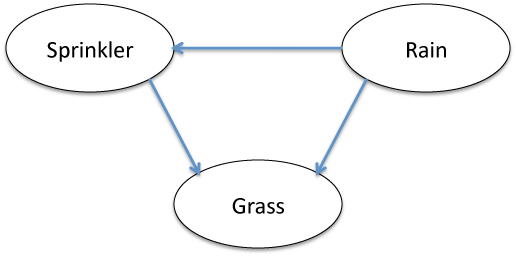
\includegraphics[width=8cm]{./images/BayesianNetwork-1.png}
					\end{answer}
				\item for each node in the network create a conditional probability table (CPT). Fill in the cells in the CPT tables with probabilities that you think are reasonable and that are not equal to 0 or 1.
					\marks{5}
					\begin{answer}
			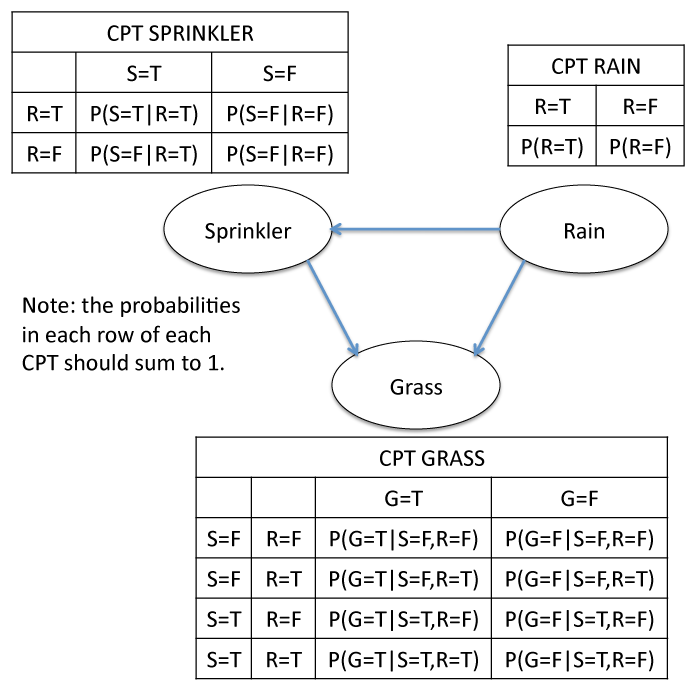
\includegraphics[width=8cm]{./images/BayesianNetwork-2.png}
					\end{answer}
				\item Using the Bayesian network and conditional probability tables you have created, compute the probability that it is raining give that the grass is wet?
					   \marks{5}
					\begin{answer}
					The answers student compute for this question will differ between students because they will each be using the probabilities they made up in step 2. However, irrespective of the specific probability values they use, they should compute $P(R=T|G=W)$ in the following manner:\\ 
					$P(R=T|G=W)=\frac{P(R=T,G=T)}{P(G=T)}=\frac{\sum_{S \in \{T,F\}} P(S, G=T, R=T)}{\sum_{S,R \in \{T,F\}} P(S, G=T, R)}$
					\end{answer}				   
		\end{enumerate}
		\item You are on holidays on Fisher Island. The yearly weather on Fisher Island comes in five different varieties: 
			\begin{itemize}
				\item there is a 10\% chance that there will be rain everyday of the year.
				\item there is a 20\% chance that there will be rain on 75\% of the days of the year.
				\item there is a 40\% chance that there will be rain on 50\% of the days of the year.
		     \item there is a 20\% chance that there will be rain on 25\% of the days of the year.
		     \item there is a 10\% chance that there will be no rain on any day of the year.
			\end{itemize}
			\begin{enumerate}
				\item given that it has rained on day 1 and 2 of the year compute the posterior probability of each of the 5 yearly weather patterns on day 2 of the year. Give your answer rounded to four places of precision.
						\marks{5}
				\begin{answer}
						To begin we will define some notation. Let: 
						\begin{itemize}
							   \item $h_1$ denote the hypothesis that it will rain everyday, $P(h_1)=0.1$.
					\item $h_2$ denote the hypothesis that it will rain on 75\% of the days of the year, with prior $P(h_2)=0.2$.
					\item $h_3$ denote the hypothesis that it will rain on 50\% of the days of the year, with prior $P(h_3)=0.4$.
					\item $h_4$ denote the hypothesis that it will rain on 25\% of the days of the year, with prior $P(h_4)=0.2$.
					\item $h_5$ denote the hypothesis that there will be no rain during the year, with prior $P(h_5)=0.1$.
					\end{itemize}
					Also, if we use the notation $rain_x$ to represent the observation of rain on day x of the year, then the probability of rain on a day of the year given a particular hypothesis $h$ is:
					\begin{itemize}
						\item $P(rain_x|h_1)=1.0$ .
						\item $P(rain_x|h_2)=0.75$ .
						\item $P(rain_x|h_3)=0.5$ .
						\item $P(rain_x|h_4)=0.25$ .
						\item $P(rain_x|h_5)=0.0$ .
					\end{itemize}
					Then:
						\begin{itemize}
							\item By Bayes' rule, we can compute the posterior probability of a hypothesis given the data so far using: $P(h_i|\textbf{d}) = \alpha P(\textbf{d}|h_i) P(h_i)$
				      		\item And, the likelihood of the data given a hypothesis is calculated using: $P(\textbf{d}|h_i) = \prod_j P(d_j|h_i)$
				           \end{itemize}
				       So:
				\begin{itemize}
					\item $P(h_1|rain_1,rain_2)=\alpha (\prod_{j=1}^2 P(rain_j|h_1))P(h_1)=\alpha 1.00^2 \times 0.1=\alpha 0.1=\frac{0.1}{0.325} \approx ..3077$.
					\item $P(h_2|rain_1,rain_2)=\alpha (\prod_{j=1}^2 P(rain_j|h_2))P(h_1)=\alpha 0.75^2 \times 0.2=\alpha 0.1125=\frac{0.1125}{0.325} \approx .3461$.
					\item $P(h_3|rain_1,rain_2)=\alpha (\prod_{j=1}^2 P(rain_j|h_3))P(h_1)=\alpha 0.50^2 \times 0.4=\alpha 0.1=\frac{0.1}{0.325} \approx ..3077$.
					\item $P(h_4|rain_1,rain_2)=\alpha (\prod_{j=1}^2 P(rain_j|h_4))P(h_1)=\alpha 0.25^2 \times 0.2=\alpha 0.0125=\frac{0.0125}{0.325} \approx .0385$.
					\item $P(h_5|rain_1,rain_2)=\alpha (\prod_{j=1}^2 P(rain_j|h_5))P(h_1)=\alpha 0.00^2 \times 0.1=\alpha 0.0=0.0$.
				\end{itemize}
			\end{answer}
				\item given that after the first 10 days of the year the weather has been such that the posterior probabilities of each of the 5 varieties of the yearly weather on Fisher Island are:  there is now a 90\% chance that there will be rain everyday for the rest of the year; a 7\% chance that there will be rain on 75\% of the rest of the days of the year;  a 2\% chance that there will be rain on 50\% of the rest of the days of the year; a 1\% chance that there will be rain on 25\% of the rest of the days of the year; and there is a 0\% chance that there will be no rain for the rest of the year.
					\begin{enumerate}
						\item what is the Bayesian Prediction probability of rain on day 11.
							   \marks{5}
					\begin{answer}
								Bayesian predictions use a likelihood-weighted sum over the hypotheses: $P(X|\textbf{d})=\sum_i P(X|h_i)P(h_i|\textbf{d})$
							     In this instance we get:\\
					$P(rain_11|\textbf{d})=\sum_i P(rain_11|h_i)P(h_i|\textbf{d})$\\
						$\qquad = (1.0 * 0.9) + (.75 * .07) + (.5 *.02) + (.25 * .01) + 0$ \\
						$\qquad = 0.9 + .0525 + 0.01 + .0025 + 0$ \\
						$\qquad = 0.965$
					\end{answer}
						\item what is the Maximum a Posterior (MAP) probability of rain on day 11.
							   \marks{5}
				         \begin{answer}
				         A MAP prediction just uses the prediction provided by the single most probable hypothesis. In this instance the single most probable hypothesis is the hypothesis that it will rain on every day of the year. This hypothesis would predict rain on day 11 with probability of 1.0 (i.e. certainty)
				         \end{answer}
				        \end{enumerate}
			\end{enumerate}
\end{enumerate}

\newpage

%Q3
%Inductive Learning (Decision Trees)
%aima chapters 18
% learning theory - supervised/unsupervised, overfitting, lazy/eager learner, classification v regression, false positive v false negatives, linear separability, consistency
% decision trees (entropy)
% knn
 \begin{table}
\begin{center}
\begin{tabular}{|c|c|c|}
$X$ & $Y$ & Class \\
\hline
T & T & + \\
T & F & - \\
T & F & + \\
T & T & + \\
F & T & - \\
\end{tabular}
\end{center}
\caption{X and Y Classification Data}
\label{tab:x-y-classification-data}
\end{table}
\question
\begin{enumerate}
\item In the context of machine learning, distinguish between \textbf{supervised} and \textbf{unsupervised} learning.
		\marks{5}
		\begin{answer}
			The distinction is that with \textbf{supervised learning} we know the actual label or category for each piece of data on which we train, whereas with \textbf{unsupervised learning} we do not know the classification of the data in the training sample. Unsupervised learning can thus often be viewed as a \textbf{clustering} task, while supervised learning can usually be seen as a \textbf{classification} task, or equivalently as a function-fitting task where one extrapolates the shape of a function based on some data points.
		\end{answer}	

	\item In the context of machine learning, explain what is meant by \textbf{overfitting} the training data.	
		\marks{5}
		\begin{answer}
			Overfitting occurs when classifiers make decisions based on accidental properties of the training set that will lead to errors on the test set (or new data). As a result, whenever there is a large set of possible hypotheses, one has to be careful not to use the resulting freedom to find meaningless "regularity" in the data.
		\end{answer}

\item Discuss the advantages and disadvantages of \textbf{$k$-Nearest Neighbour} classification.
				\marks{10}
				\begin{answer}
				Strengths
				\begin{enumerate}	
					\item No training involved � lazy learning
					\item New data can be added on the fly
					\item Some explanation capabilities
					\item Robust to noisy data by averaging k-nearest neighbors
				\end{enumerate}
				Weaknesses
				\begin{enumerate}
					\item Not the most powerful classification (generally its accuracy will be lower than an ANN or SVM model)
					\item Slow classification 
					\item Curse of dimensionality (as you increase the number of features you need more and more examples to cover the problem space - kNN are particularly susceptible to this issue as they do not do any feature selection).
				\end{enumerate}
			\end{answer}	

%Callan Chapter 12 Q.3
\item Table \ref{tab:x-y-classification-data} provides a classification for a data set of X Y pairs.
	\begin{enumerate}
	\item Calculate the \textbf{entropy} for this classification.
	\marks{5}
	\begin{answer}
		Entropy is $-\frac{3}{5}log_2\frac{3}{5}-\frac{2}{5}log_2\frac{2}{5}=0.971$
	\end{answer}
	\item Calculate the \textbf{information gain} for X and Y.
	\marks{5}
	\begin{answer}
		Entropy for X = T $-\frac{3}{4}log_2\frac{3}{4}-\frac{1}{4}log_2\frac{1}{4}=0.811$\\
		Entropy for X = F $0-\frac{1}{1}log_2\frac{1}{1}=0$\\
		Gain for X $0.971-(\frac{4}{5}\times0.811+\frac{1}{5}\times0)=0.322$\\
		Entropy for Y = T $-\frac{2}{3}log_2\frac{2}{3}-\frac{1}{3}log_2\frac{1}{3}=0.918$\\
		Entropy for Y = F $-\frac{1}{2}log_2\frac{1}{2}-\frac{1}{2}log_2\frac{1}{2}=1.0$\\
		Gain for Y $0.971-(\frac{3}{5}\times0.918+\frac{2}{5}\times1)=0.02$\\
	\end{answer}
	\end{enumerate}
\end{enumerate}

\newpage

%Q4
%Linear Regression Neural Nets, SVMs, Ensemble Learning
%Inductive Logic programming
\question Figure \ref{fig:nn} shows a backprogation network that is currently processing the training vector $[1.0, 0.9, 0.9]$ which has an  associated target vector $[0.1, 0.9, 1.0]$. Given that the output from unit B is $0.6$ and from C is $0.8$, and assuming that the activation function used at all nodes in the network is the logistic function (i.e., $f(x) = \frac{1}{1 + \exp^{-x}}$): 
\begin{enumerate}
	\item Calculate the actual output vector (to 3 decimal places).
		\marks{5}
		\begin{answer}
		Output of unit $i = f(\sum_{j=1}^{n}W_{j,i}\times activation_j)$\\
		First output unit input = -0.3 x 0.6 + 0.9 x 0.8 = 0.54 $\rightarrow$ f(0.54) = 0.632\\
		Second output unit input = -0.6 x 0.6 + -0.1 x 0.8 = -0.44 $\rightarrow$ f(-0.44) = 0.392\\
		Third output unit input = 0.4 x 0.6 + 1.2 x 0.8 = 1.2 $\rightarrow$ f(1.2)= 0.769\\
		\end{answer}
	\item Calculate the error for each output unit.
		\marks{5}
		\begin{answer}
		Error =  target - output\\
		First output unit = (0.1 - 0.632)  = - 0.532\\
		Second output unit = (0.9 - 0.392) = 0.508\\
		Third output unit = (0.1 - 0.769) = - 0.696\\
		\end{answer}
	\item Calculate the error for each hidden unit B and C.
		\marks{10}
		\begin{answer}
		Each hidden node $j$ is responsible for some fraction of the error $Err_i$ of each of the output units $i$ to which it connects. Thus the $Err_i$ values are divided according to the strengths of the connection between the hidden node and the output nodes and are propagated back to the hidden nodes. Where a hidden node feeds-forward into more than 1 output node the errors propagated back to it are summed: $Err_j = \sum_{i=1}^{n}W_{ji} \times Err_i$:
		$Err_{B} = (-0.3 \times -0.532) + (-0.6 \times 0.508) + (0.4 \times -0.696) = 0.1596 + -0.3048 + -0.2784 = -0.4236$\\
		$Err_{C} = (0.9 \times -0.532) + (-0.1 \times 0.508) + (1.2 \times -0.696) =  -0.4788 + -0.0508 + -0.8352  = -1.3648$\\
		\end{answer}		
	\item The following sets express the mappings between predicates $r$, $p$, $q$, $s$, $class1$ and $class2$: $r\rightarrow \{a1, a2, a5, a6 \}$, $p\rightarrow \{a2, a3, a5, a7 \}$, $q\rightarrow \{a1, a2, a6 \}$, $s\rightarrow \{(a2, f), (a1,1), (a6,f)\}$, $class1\rightarrow \{a2\}$, $class2\rightarrow \{a2, a6\}$.
\begin{enumerate}
	\item Given the above sets give a specialisation of the rule $class1(X)\leftarrow r(X) \land p(X)$ such that the rule is only satisfied by $class1$ members.
	\marks{5}
	\begin{answer}
	$class1(X)\leftarrow r(X) \land p(X) \land q(X)$
	\end{answer}
	\item Given the above sets give a rule that will correctly classify only members of $class2$.
	\marks{5}
	\begin{answer}
	$class2(X)\leftarrow s(X, f)$
	\end{answer}
\end{enumerate}

\end{enumerate}

\begin{figure}[htbp]
\begin{center}
\includegraphics[width=3.5in]{./images/nn_callan_q10_2.png}
\caption{Example Neural Net}
\label{fig:nn}
\end{center}
\end{figure}


\end{document}
